\documentclass{beamer}
\setbeamertemplate{footline}[frame number]
%\usepackage{beamerthemeBerkeley}
\usetheme{Montpellier}
%\usetheme{Warsaw}
%\usetheme{Boadilla}
\usepackage[english]{babel}
\usepackage{graphicx}
\usepackage[font=small,labelfont=bf]{caption} % Required for specifying captions to tables and figures
%\usepackage{ams}
%\usepackage{blue}
\captionsetup{labelformat=empty,labelsep=none}

\title [Introduction to Association Mapping Module] {  \fontsize{12}{15}\selectfont Association Mapping: GWAS and Sequencing Data } 

\author{Instructors: Joelle Mbatchou and Loic Yengo}

\date{}






\begin{document}

\begin{frame}
\titlepage
\vspace{-2cm}
\begin{center}
{ \large Summer Institute in Statistical Genetics (SISG) \\}
\vspace{.3cm}
 {\large July 2022 \\}
\vspace{.8cm}
\end{center}
\end{frame}



\begin{frame}
\frametitle{\bf Introduction: Course Goals}
This is a course on statistical methods and software for genetic association studies of complex traits. We aim to cover:
{\small
\begin{itemize}
\item Genetic Association Testing with Case-Control  \& Quantitative Traits
\item Population Structure/Ancestry Inference 
\item Genetic Association Testing in Samples with Structure
\item Conditional analyses, Colocalization, Fine-mapping \& Polygenic Risk Scores
\item Gene and Pathway Level Analysis 
\item Association Testing for Rare Variant Analysis
\item Interaction Analysis, GWAX, Time-to-event \& Multi-trait Analysis
\item Power and Sample Size, Design Considerations and Emerging Issues
\end{itemize}
}
\end{frame}


\begin{frame}[fragile]
\frametitle{\bf Introduction: Resources}

Importantly, the class site is: 
{\color{red}
 
\url{https://joellembatchou.github.io/SISG2022_Association_Mapping/}

}
\vspace{.3cm}
Contains (or will contain):
\begin{itemize}
\item Link to PDF copies of slides
\item Practical exercises for you to try
\item Link to datasets used in exercises
\item Our solutions to exercises (later!)
\item Links to software packages
\end{itemize}
\end{frame}


\begin{frame}
\frametitle{Introduction: About Loic}
\begin{tabular}{cc}
\raisebox{.1in}{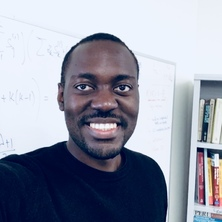
\includegraphics[scale=.5]{Figures/Loic_Yengo.jpeg}} &
\raisebox{1.2in}{
\begin{minipage}{6in}
\begin{itemize}
\item A
\item B
\item C
\end{itemize}
\end{minipage}
}
\end{tabular}
\end{frame}


    


\begin{frame}
\frametitle{Introduction: About Joelle}
\begin{tabular}{cc}
\raisebox{.03in}{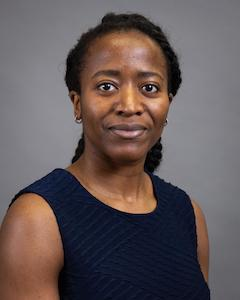
\includegraphics[scale=.4]{Figures/Joelle_Mbatchou.jpeg}} &
\raisebox{.9in}{
\begin{minipage}{7in}
\begin{itemize}
\item Statistical Geneticist, \\Regeneron Genetics Center
\item Research in: \\
\begin{itemize}
\item     Genetic Association Studies\\
\item     Genetic Data with Structure\\
\item	Mixed Models methods\\
\item	Association methods for large-scale\\ datasets\\
\end{itemize}
\end{itemize}
\end{minipage}
}
\end{tabular}
\end{frame}


\begin{frame}


\begin{center}
	\captionof{figure}{\textit{\bf UW  department's finest -- here to help you!}}
	\begin{minipage}{0.32\linewidth}
		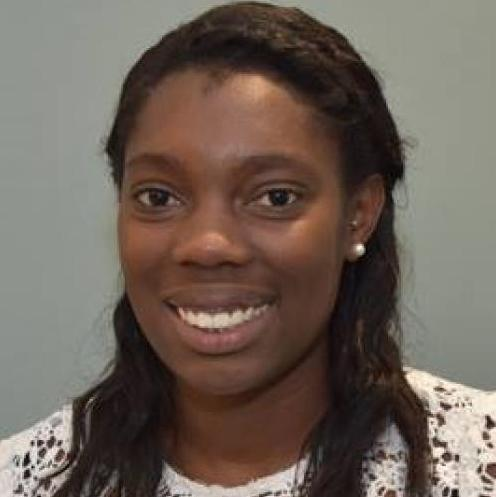
\includegraphics[width=\linewidth,height=\linewidth]{Figures/Amarise-little.jpg}
		\captionof{figure}{Amarise Little}
	\end{minipage}
	\begin{minipage}{0.32\linewidth}
		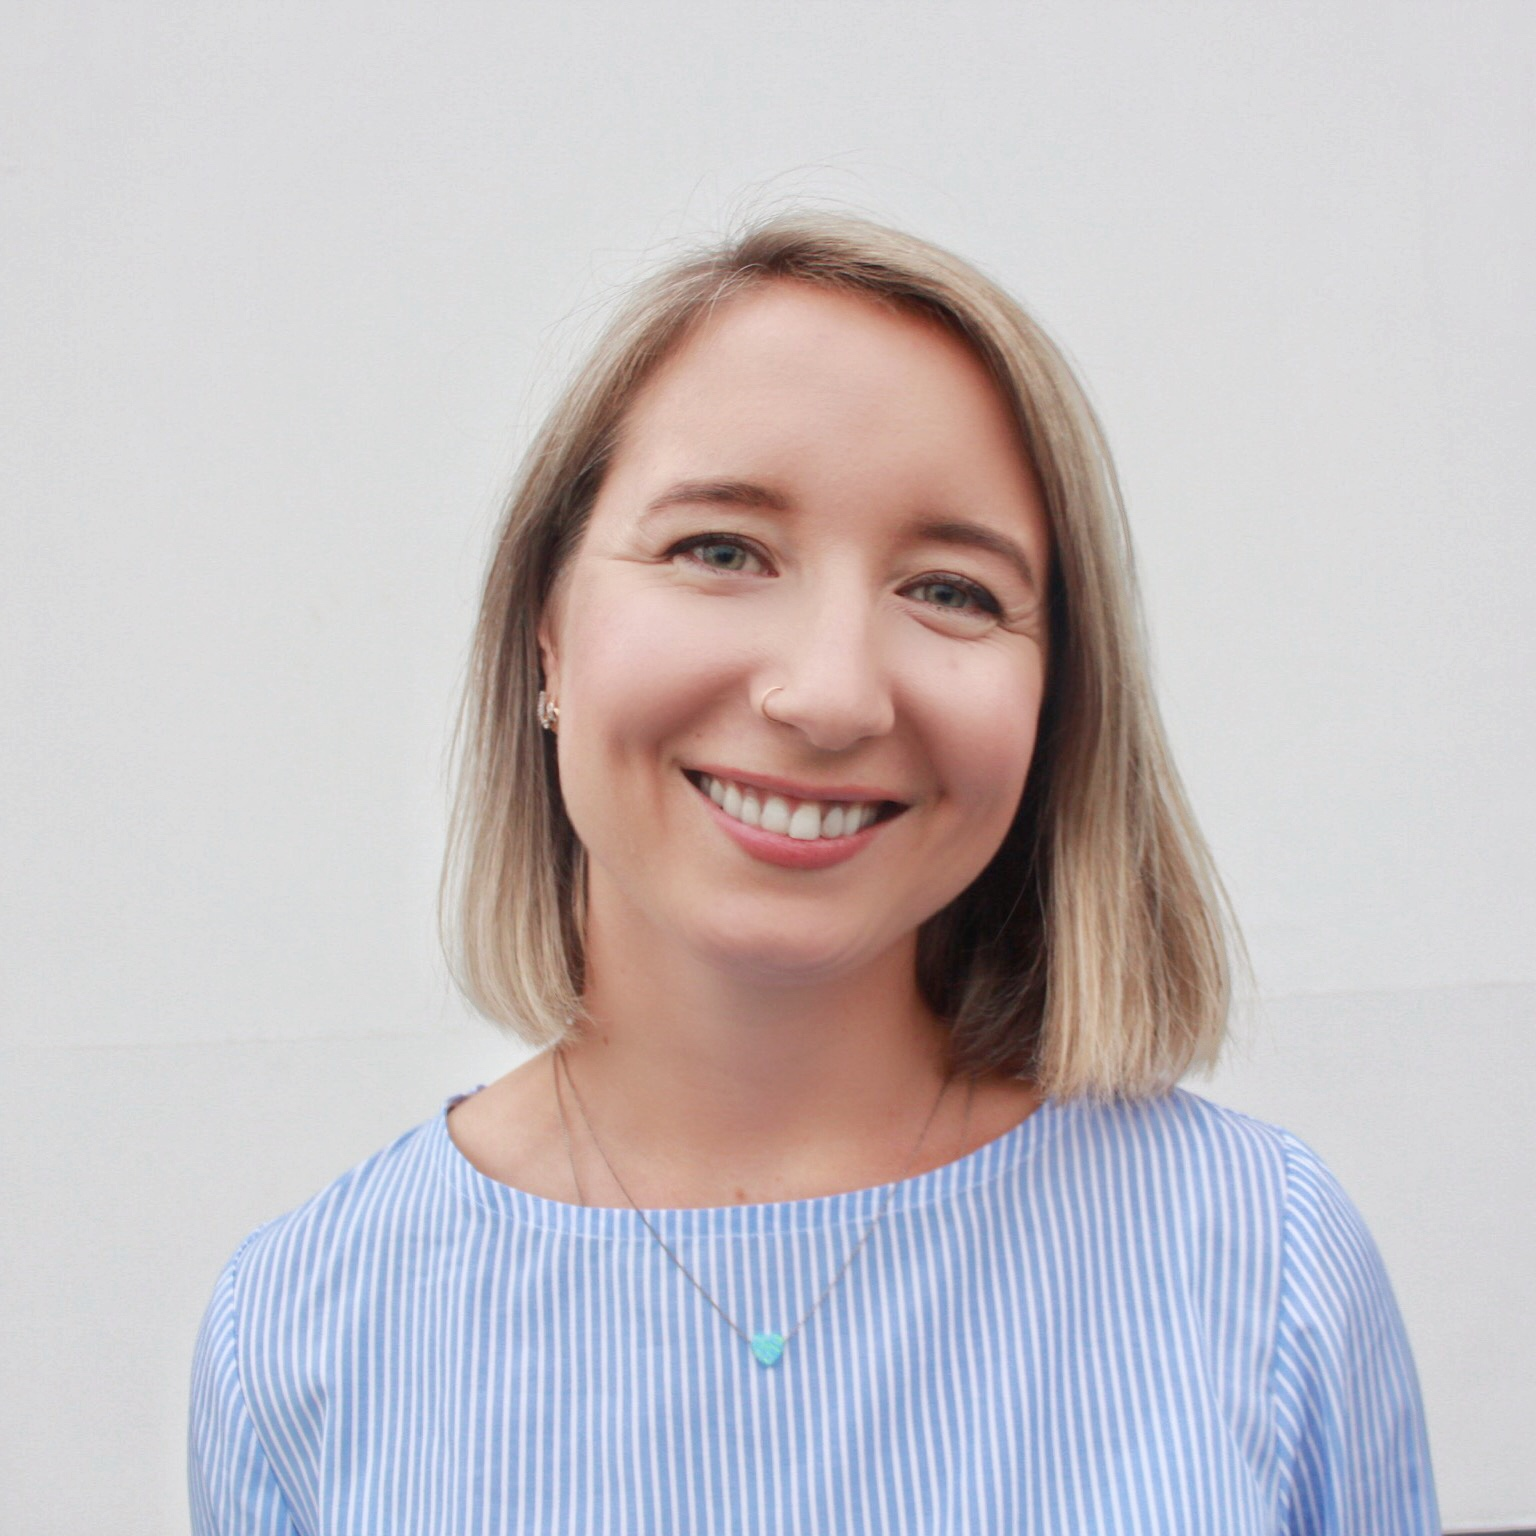
\includegraphics[width=\linewidth,height=\linewidth]{Figures/anyamikhaylova.jpg}
		\captionof{figure}{Anya Mikhaylova}
	\end{minipage}
	\hfill
	\begin{minipage}{0.32\linewidth}
		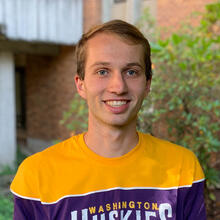
\includegraphics[width=\linewidth,height=\linewidth]{Figures/seth-temple.jpeg}
		\captionof{figure}{Seth Temple}
	\end{minipage}
\end{center}

%\begin{center}
%    \begin{tabular}{cccc}
%Andrea Horimoto &  Amarise Little &
% Anya Mikhaylova & Seth Temple \\
%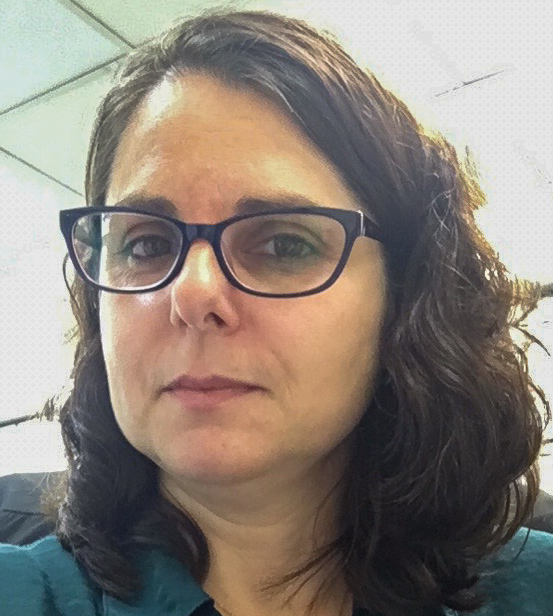
\includegraphics[scale=.3]{Figures/Andrea.jpg} & 
%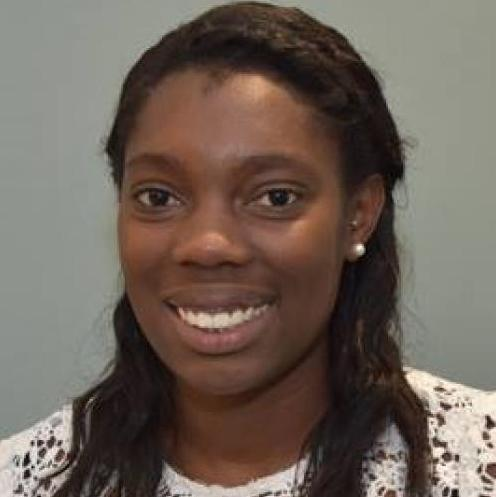
\includegraphics[scale=.3]{Figures/Amarise-little.jpg} 
%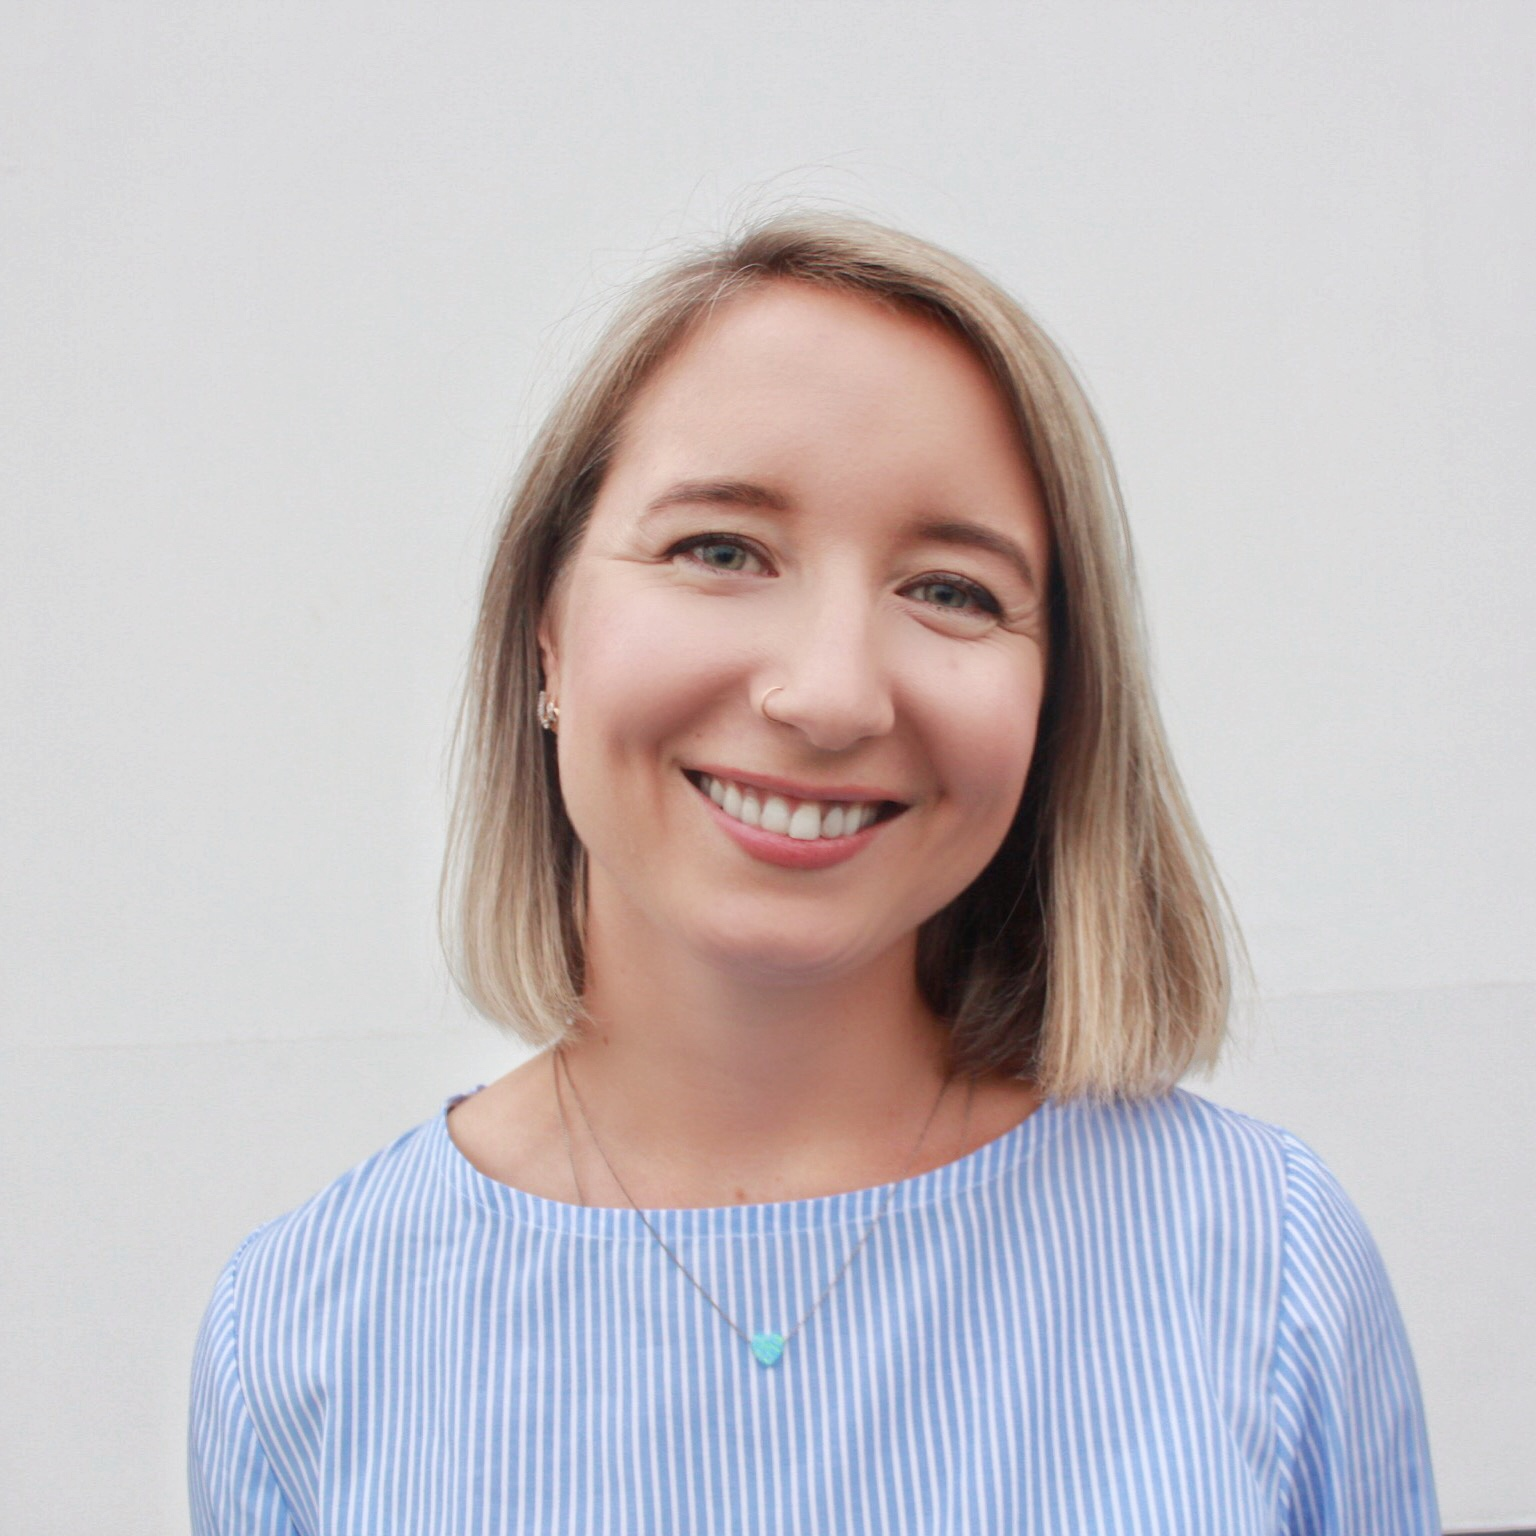
\includegraphics[scale=.05]{Figures/anyamikhaylova.jpg} &
%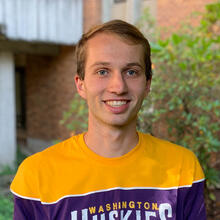
\includegraphics[scale=.5]{Figures/seth-temple.jpeg}
%\end{tabular}
%\end{center}
\end{frame}



\begin{frame}[fragile]
\frametitle{\bf Slack Channel}

Expect to `see' them on Zoom chat, and our Slack channel:
{\color{red}
 
\url{https://uwbiostatisticssisg.slack.com/archives/C03KLGA4HE3}


}
\vspace{.3cm}
Contains (or will contain);
\begin{itemize}
\item Key annoucements
\item Link to the class website
\item PDF copies of slides
\item Link to practical exercises
\end{itemize}
\end{frame}



\begin{frame}[fragile]
	\frametitle{\bf Cloud server}
	
	We will use a cloud server to do the practical exercises. 
	For more info on  getting set up on the server:
	{\color{red}
		\url{https://joellembatchou.github.io/SISG2022_Association_Mapping/using_server.html}
%		\verb+ssh -XY <username>@si2022-m15.biostat.washington.edu+
	}

	\vspace{1em}
	Things to note:
	\begin{itemize}
		\item {\bf Let us know if you cannot access the server}
		\item We will run command line exercises on the server
		\item Check the course website for details on where the datasets are for each session
	\end{itemize}
\end{frame}







\begin{frame}
\frametitle{\bf Introduction: Course Structure}
\begin{itemize}
\item 10 sessions, 60-90 minutes each, over 2.5 days
\item What to expect in a typical session;
\begin{itemize} 
\item 45 mins teaching/lecture 
\item 30 mins hands-on exercises
\item 15 mins summary/discussion
\end{itemize}
\end{itemize}
\end{frame}




\end{document}

